% Options for packages loaded elsewhere
\PassOptionsToPackage{unicode}{hyperref}
\PassOptionsToPackage{hyphens}{url}
%
\documentclass[
]{article}
\usepackage{amsmath,amssymb}
\usepackage{iftex}
\ifPDFTeX
  \usepackage[T1]{fontenc}
  \usepackage[utf8]{inputenc}
  \usepackage{textcomp} % provide euro and other symbols
\else % if luatex or xetex
  \usepackage{unicode-math} % this also loads fontspec
  \defaultfontfeatures{Scale=MatchLowercase}
  \defaultfontfeatures[\rmfamily]{Ligatures=TeX,Scale=1}
\fi
\usepackage{lmodern}
\ifPDFTeX\else
  % xetex/luatex font selection
\fi
% Use upquote if available, for straight quotes in verbatim environments
\IfFileExists{upquote.sty}{\usepackage{upquote}}{}
\IfFileExists{microtype.sty}{% use microtype if available
  \usepackage[]{microtype}
  \UseMicrotypeSet[protrusion]{basicmath} % disable protrusion for tt fonts
}{}
\makeatletter
\@ifundefined{KOMAClassName}{% if non-KOMA class
  \IfFileExists{parskip.sty}{%
    \usepackage{parskip}
  }{% else
    \setlength{\parindent}{0pt}
    \setlength{\parskip}{6pt plus 2pt minus 1pt}}
}{% if KOMA class
  \KOMAoptions{parskip=half}}
\makeatother
\usepackage{xcolor}
\usepackage{longtable,booktabs,array}
\usepackage{calc} % for calculating minipage widths
% Correct order of tables after \paragraph or \subparagraph
\usepackage{etoolbox}
\makeatletter
\patchcmd\longtable{\par}{\if@noskipsec\mbox{}\fi\par}{}{}
\makeatother
% Allow footnotes in longtable head/foot
\IfFileExists{footnotehyper.sty}{\usepackage{footnotehyper}}{\usepackage{footnote}}
\makesavenoteenv{longtable}
\usepackage{graphicx}
\makeatletter
\def\maxwidth{\ifdim\Gin@nat@width>\linewidth\linewidth\else\Gin@nat@width\fi}
\def\maxheight{\ifdim\Gin@nat@height>\textheight\textheight\else\Gin@nat@height\fi}
\makeatother
% Scale images if necessary, so that they will not overflow the page
% margins by default, and it is still possible to overwrite the defaults
% using explicit options in \includegraphics[width, height, ...]{}
\setkeys{Gin}{width=\maxwidth,height=\maxheight,keepaspectratio}
% Set default figure placement to htbp
\makeatletter
\def\fps@figure{htbp}
\makeatother
\setlength{\emergencystretch}{3em} % prevent overfull lines
\providecommand{\tightlist}{%
  \setlength{\itemsep}{0pt}\setlength{\parskip}{0pt}}
\setcounter{secnumdepth}{-\maxdimen} % remove section numbering
% Configuración de márgenes y diseño
\usepackage[top=2.5cm,bottom=2.5cm,left=2.5cm,right=2.5cm]{geometry}
\usepackage{setspace}
\setstretch{1.15}

% Soporte para caracteres Unicode (modo una columna)
\usepackage{newunicodechar}
\usepackage{array}
\usepackage{longtable}
\usepackage{booktabs}
\usepackage{tabularx}
\usepackage{ragged2e}

% Definir caracteres Unicode problemáticos
\newunicodechar{₀}{\ensuremath{_0}}
\newunicodechar{₁}{\ensuremath{_1}}
\newunicodechar{₂}{\ensuremath{_2}}
\newunicodechar{₃}{\ensuremath{_3}}
\newunicodechar{₄}{\ensuremath{_4}}
\newunicodechar{₅}{\ensuremath{_5}}
\newunicodechar{₆}{\ensuremath{_6}}
\newunicodechar{₇}{\ensuremath{_7}}
\newunicodechar{₈}{\ensuremath{_8}}
\newunicodechar{₉}{\ensuremath{_9}}
\newunicodechar{⁺}{\ensuremath{^+}}
\newunicodechar{⁻}{\ensuremath{^-}}
\newunicodechar{°}{\textdegree}
\newunicodechar{×}{\texttimes}
\newunicodechar{·}{\textperiodcentered}
\newunicodechar{–}{\textendash}
\newunicodechar{—}{\textemdash}
\newunicodechar{λ}{\ensuremath{\lambda}}
\newunicodechar{σ}{\ensuremath{\sigma}}
\newunicodechar{ε}{\ensuremath{\varepsilon}}
\newunicodechar{μ}{\ensuremath{\mu}}
\newunicodechar{χ}{\ensuremath{\chi}}
\newunicodechar{α}{\ensuremath{\alpha}}
\newunicodechar{β}{\ensuremath{\beta}}
\newunicodechar{γ}{\ensuremath{\gamma}}
\newunicodechar{δ}{\ensuremath{\delta}}
\newunicodechar{θ}{\ensuremath{\theta}}
\newunicodechar{φ}{\ensuremath{\phi}}
\newunicodechar{ω}{\ensuremath{\omega}}
\newunicodechar{π}{\ensuremath{\pi}}
\newunicodechar{Σ}{\ensuremath{\Sigma}}
\newunicodechar{Δ}{\ensuremath{\Delta}}
\newunicodechar{∞}{\ensuremath{\infty}}
\newunicodechar{≈}{\ensuremath{\approx}}
\newunicodechar{≠}{\ensuremath{\neq}}
\newunicodechar{≤}{\ensuremath{\leq}}
\newunicodechar{≥}{\ensuremath{\geq}}
\newunicodechar{→}{\ensuremath{\rightarrow}}
\newunicodechar{←}{\ensuremath{\leftarrow}}
\newunicodechar{↔}{\ensuremath{\leftrightarrow}}
\newunicodechar{↑}{\ensuremath{\uparrow}}
\newunicodechar{↓}{\ensuremath{\downarrow}}
\newunicodechar{±}{\ensuremath{\pm}}
\newunicodechar{÷}{\ensuremath{\div}}
\newunicodechar{≪}{\ensuremath{\ll}}
\newunicodechar{≫}{\ensuremath{\gg}}
\newunicodechar{∇}{\ensuremath{\nabla}}
\newunicodechar{∂}{\ensuremath{\partial}}

% Configuración para tablas
\setlength{\LTpre}{\baselineskip}
\setlength{\LTpost}{\baselineskip}
\renewcommand{\arraystretch}{1.2}

% Permitir que las tablas se ajusten al ancho de página
\makeatletter
\def\tabularxcolumn#1{m{#1}}
\makeatother
\ifLuaTeX
  \usepackage{selnolig}  % disable illegal ligatures
\fi
\usepackage{bookmark}
\IfFileExists{xurl.sty}{\usepackage{xurl}}{} % add URL line breaks if available
\urlstyle{same}
\hypersetup{
  hidelinks,
  pdfcreator={LaTeX via pandoc}}

\author{}
\date{}

\begin{document}

\section{Impacto de la estimulación electromagnética en las propiedades
mecánicas y la calidad del grano de trigo de
invierno}\label{impacto-de-la-estimulaciuxf3n-electromagnuxe9tica-en-las-propiedades-mecuxe1nicas-y-la-calidad-del-grano-de-trigo-de-invierno}

\textbf{Autores:} A. Dziwulska-Hunek, K. Sadowski, M. Kania, K.
Krawczyk, J. Wowro\\
\textbf{Revista:} Scientific Reports (Nature)\\
\textbf{Año:} 2022\\
\textbf{DOI:} \url{https://doi.org/10.1038/s41598-022-20737-z}

\begin{center}\rule{0.5\linewidth}{0.5pt}\end{center}

\section{Materiales y métodos}\label{materiales-y-muxe9todos}

\begin{quote}
\textbf{Material vegetal.} El material de investigación consistió en
hojas de alfalfa de 4 años de edad, cultivar Ulstar, obtenidas del
experimento de campo conducido por el Departamento de Tecnología de
Producción Vegetal y Ciencia de Productos Básicos, Universidad de
Ciencias de la Vida, en Felin (51°13′21.9″ N, 22°37′55.85″ E), en un
suelo clasificado en el complejo bueno de trigo (clase de calidad de
suelo III a). Las hojas se cosecharon el 25 de mayo de 2018, durante la
fase de botones florales (escala BBCH 55--59).
\end{quote}

\begin{quote}
\textbf{Estimulación electromagnética.} Las hojas crecieron a partir de
semillas sometidas a tratamiento previo a la siembra: C
(control---semillas no estimuladas); L1 y L5---semillas estimuladas con
luz láser con 1 y 5 minutos de exposición, respectivamente; y F1 y
F5---semillas estimuladas con un campo magnético con 1 y 5 minutos de
exposición, respectivamente.
\end{quote}

\begin{quote}
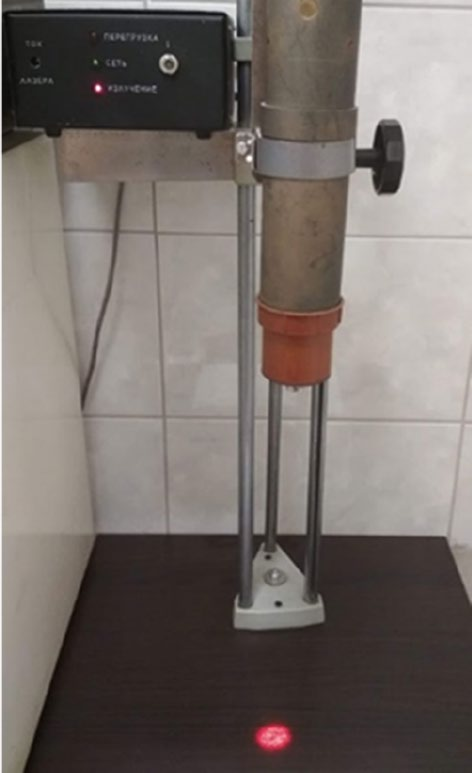
\includegraphics{./images/figure1-laser-rig.jpg}
\end{quote}

\begin{quote}
\textbf{Figura 1.} Dispositivo diseñado para estimulación láser de
semillas. Foto de Agata Dziwulska-Hunek.
\end{quote}

La estimulación con luz se realizó utilizando un láser He-Ne con
longitud de onda de 632,8 nm y densidad de potencia superficial de 3 mW
cm⁻². Se creó un dispositivo propietario y único para este propósito
(Figura 1), con el haz de luz láser divergente dirigido hacia abajo
sobre semillas colocadas en una sola capa en el fondo de una placa. Se
utilizó un electroimán (Figura 2) {[}23{]} para estimular las semillas
con un campo magnético alterno con inducción magnética de 30 mT.

\begin{quote}
\textbf{Resistencia mecánica de las hojas.} La prueba de tensión se
realizó utilizando un instrumento Zwick/Roell Z005 equipado con software
de registro de datos Test Xpert II.V3.5 de Zwick. La tensión se aplicó
utilizando una cabeza de medición de 50 N a una velocidad de 10 mm s⁻¹
(Figuras {[}3{]} y {[}4{]}). La temperatura en el laboratorio se mantuvo
a
\end{quote}

\begin{quote}

\includegraphics{./images/image16.jpeg}
\end{quote}

\textbf{Figura 2.} Electromagneto. Foto de Agata Dziwulska-Hunek.


\includegraphics{./images/image17.jpeg}

\textbf{Figura 3.} Antes y después de la tensión con el instrumento
Zwick/Roell Z005. Foto de Agata Dziwulska-Hunek.


\includegraphics{./images/image18.jpeg}

\textbf{Figura 4.} Una hoja antes y después de la tensión. Foto de Agata
Dziwulska-Hunek.

\begin{quote}
20 °C durante la medición. Las hojas probadas se recolectaron de las
partes superior, media e inferior de los tallos de las plantas (Figura
{[}5{]}). Cada medición de muestra se repitió cinco veces.
\end{quote}

\begin{quote}
\textbf{Tiempos de vida de fluorescencia.} Las mediciones de decaimiento
de fluorescencia se realizaron utilizando un fluorímetro de modulación
de fase K2 (ISS, EE.UU.). Las hojas se trituraron en un mortero en un
amortiguador Hepes--NaOH (25 mM; pH 7,8) que contenía 1 mM de MgCl₂, 1
mM de EDTA y 0,4 M de sorbitol.
\end{quote}

\begin{quote}

\includegraphics{./images/image19.jpeg}
\end{quote}

\textbf{Figura 5.} Partes del tallo de las cuales se recolectaron hojas
para análisis. Foto de Agata Dziwulska-Hunek.

\begin{quote}
El homogenato se diluyó utilizando el amortiguador de modo que la
absorbancia de la muestra a 440 nm no excediera 0,15. La muestra se
excitó con ondas de 440 nm y la fluorescencia se observó a través de un
filtro de corte KV550 (λ \textgreater{} 550 nm). Las mediciones se
realizaron en una cubeta de 1 × 1 cm, a temperatura ambiente, a 10
frecuencias de modulación de onda excitadora (en el rango de 2--200
MHz), relativas a la suspensión difusora (Ludox®, Sigma Aldrich). Se
utilizó el software Vinci2 (ISS, EE.UU.) en el análisis para un modelo
de decaimiento de fluorescencia exponencial doble y triple que mejor
correspondiera a los resultados obtenidos. Todas las mediciones se
realizaron por triplicado.
\end{quote}

\begin{quote}
\textbf{Pigmentos fotosintéticos.} Determinación del contenido de
pigmentos fotosintéticos. Los pigmentos fotosintéticos se aislaron de
las hojas utilizando acetona que contenía 0,01\% p/v de BHT (butil
hidroxitolueno), en oscuridad, después de lo cual se determinaron los
contenidos de clorofila y carotenoides. El espectro UV-Vis se midió
utilizando un espectrómetro Carry Bio 300 y se analizó de acuerdo con el
procedimiento publicado por Lichtenthaler y Buschmann {[}24{]}. Cada
muestra se analizó por triplicado.
\end{quote}

\begin{quote}
\textbf{Análisis estadístico.} Los resultados experimentales se
procesaron con el software STATISTICA 13,1, utilizando el análisis de
varianza ANOVA y la prueba post-hoc LSD al nivel de significancia de α =
0,05. Las relaciones entre variables se determinaron utilizando el
coeficiente de correlación lineal de Pearson.
\end{quote}

\begin{quote}
Confirmamos que los estudios experimentales y de campo sobre las plantas
cultivadas en el estudio cumplen con las directrices institucionales y
nacionales relevantes y la legislación vigente en el Centro de
Investigación para Pruebas de Cultivares {[}25{]}.
\end{quote}

\section{Resultados y discusión}\label{resultados-y-discusiuxf3n}

\begin{quote}
\textbf{Resistencia mecánica a la tensión.} Los parámetros de las hojas
medidos antes de la prueba de resistencia a la tensión incluyeron el
largo y el ancho de la hoja y el grosor del pecíolo, así como la masa de
la hoja sin el pecíolo medida después de la prueba, se presentan en la
Tabla {[}1{]}. La prueba de tensión midió la fuerza necesaria para
desprender la hoja del pecíolo (Tabla {[}2{]}). En general, la
estimulación de semillas no afectó significativamente los parámetros
probados. Sin embargo, se observó cierta reducción de los mismos para
las secciones superior y media del tallo. Por otro lado, las hojas de la
parte inferior del tallo mostraron resultados contrarios con el largo de
la hoja y el grosor del pecíolo visiblemente aumentados debido a la
estimulación del campo electromagnético.
\end{quote}

\begin{quote}
Los datos sobre los parámetros registrados después de desgarrar las
hojas que crecieron a partir de semillas sometidas a estimulación
electromagnética se presentan en la Tabla {[}2{]}. La resistencia a la
tensión de las hojas se midió en aproximadamente 1,58--2,45 N. La
estimulación electromagnética redujo la resistencia a la tensión de las
hojas que se recolectaron de las partes superior e inferior del tallo,
especialmente para L5 y F5. La disminución significativa se observó para
el tratamiento L5 para la parte superior del tallo, donde el valor fue
del 73\% en relación con el control. Se observó un ligero aumento de
este parámetro para las hojas inferiores. La diferencia observada puede
deberse a las dimensiones de las hojas o al grosor del tallo, o
posiblemente a la forma general de las hojas. Se observó una interacción
entre las variables L5 y F1, L5 y F5. Debe señalarse que la masa de las
hojas sin pecíolos (de la parte superior) fue mayor en el objeto
estimulado L5, en comparación con los objetos F1 y F5. A su vez, el
grosor del pecíolo y la resistencia a la tensión se redujeron.
\end{quote}

\begin{longtable}[]{@{}
  >{\raggedright\arraybackslash}p{(\columnwidth - 6\tabcolsep) * \real{0.2564}}
  >{\raggedright\arraybackslash}p{(\columnwidth - 6\tabcolsep) * \real{0.2564}}
  >{\raggedright\arraybackslash}p{(\columnwidth - 6\tabcolsep) * \real{0.2308}}
  >{\raggedright\arraybackslash}p{(\columnwidth - 6\tabcolsep) * \real{0.2564}}@{}}
\toprule\noalign{}
\begin{minipage}[b]{\linewidth}\raggedright
\textbf{Factores de estimulación}
\end{minipage} & \begin{minipage}[b]{\linewidth}\raggedright
\textbf{Parte superior del tallo}
\end{minipage} & \begin{minipage}[b]{\linewidth}\raggedright
\textbf{Parte media del tallo}
\end{minipage} & \begin{minipage}[b]{\linewidth}\raggedright
\textbf{Parte inferior del tallo}
\end{minipage} \\
\midrule\noalign{}
\endhead
\bottomrule\noalign{}
\endlastfoot
\textbf{Largo (cm)} & & & \\
C & 3,00 ± 0,49a & 3,18 ± 0,62a & 2,14 ± 0,29a \\
L1 & 3,20 ± 0,12a & 3,22 ± 0,55a & 2,30 ± 0,88a \\
L5 & 2,84 ± 0,29a & 3,18 ± 0,18a & 2,00 ± 0,45a \\
F1 & 2,80 ± 0,12a & 2,94 ± 0,30a & 2,66 ± 0,50a \\
F5 & 2,94 ± 0,43a & 2,98 ± 0,51a & 2,60 ± 0,27a \\
\textbf{Ancho (cm)} & & & \\
C & 1,30 ± 0,32a & 1,76 ± 0,32a & 1,38 ± 0,51a \\
L1 & 1,32 ± 0,15a & 1,64 ± 0,22a & 1,59 ± 0,62a \\
L5 & 1,06 ± 0,23a & 1,54 ± 0,22a & 1,34 ± 0,06a \\
F1 & 1,24 ± 0,25a & 1,38 ± 0,16a & 1,40 ± 0,24a \\
F5 & 1,30 ± 0,34a & 1,76 ± 0,69a & 1,76 ± 0,47a \\
\textbf{Grosor del pecíolo (mm)} & & & \\
C & 0,548 ± 0,190a & 0,660 ± 0,173a & 0,368 ± 0,204a \\
L1 & 0,540 ± 0,073a & 0,592 ± 0,198a & 0,456 ± 0,247a \\
L5 & 0,432 ± 0,061a & 0,656 ± 0,069a & 0,364 ± 0,092a \\
F1 & 0,484 ± 0,063a & 0,666 ± 0,150a & 0,444 ± 0,125a \\
F5 & 0,506 ± 0,245a & 0,624 ± 0,237a & 0,542 ± 0,235a \\
\textbf{Masa de hoja sin pecíolo (g)} & & & \\
C & 0,713 ± 0,084a & 0,803 ± 0,123a & 0,632 ± 0,137a \\
L1 & 0,769 ± 0,034a & 0,821 ± 0,096a & 0,691 ± 0,193a \\
L5 & 0,743 ± 0,090a & 0,790 ± 0,085a & 0,651 ± 0,094a \\
F1 & 0,668 ± 0,084a & 0,802 ± 0,081a & 0,647 ± 0,059a \\
F5 & 0,702 ± 0,109a & 0,750 ± 0,062a & 0,735 ± 0,084a \\
\end{longtable}

\textbf{Tabla 1.} Parámetros que caracterizan las hojas de alfalfa.
\emph{C} control (semillas no estimuladas); \emph{L1, L5} estimulación
con luz láser He-Ne con 1 y 5 minutos de exposición, respectivamente;
\emph{F1, F5} estimulación con campo magnético alterno con 1 y 5 minutos
de exposición, respectivamente. a, b---letras diferentes en columnas
respectivas indican diferencias estadísticas, ± desviación estándar, n =
5.

\begin{longtable}[]{@{}
  >{\raggedright\arraybackslash}p{(\columnwidth - 6\tabcolsep) * \real{0.2564}}
  >{\raggedright\arraybackslash}p{(\columnwidth - 6\tabcolsep) * \real{0.2564}}
  >{\raggedright\arraybackslash}p{(\columnwidth - 6\tabcolsep) * \real{0.2308}}
  >{\raggedright\arraybackslash}p{(\columnwidth - 6\tabcolsep) * \real{0.2564}}@{}}
\toprule\noalign{}
\begin{minipage}[b]{\linewidth}\raggedright
\textbf{Factores de estimulación}
\end{minipage} & \begin{minipage}[b]{\linewidth}\raggedright
\textbf{Parte superior del tallo}
\end{minipage} & \begin{minipage}[b]{\linewidth}\raggedright
\textbf{Parte media del tallo}
\end{minipage} & \begin{minipage}[b]{\linewidth}\raggedright
\textbf{Parte inferior del tallo}
\end{minipage} \\
\midrule\noalign{}
\endhead
\bottomrule\noalign{}
\endlastfoot
\textbf{Fuerza (N)} & & & \\
C & 2,16 ± 0,48a & 2,45 ± 0,53a & 1,59 ± 0,62a \\
L1 & 2,32 ± 0,13a & 2,36 ± 0,48a & 1,77 ± 1,00a \\
L5 & 1,58 ± 0,20bd & 2,12 ± 0,20a & 1,65 ± 0,45a \\
F1 & 1,79 ± 0,25ac & 2,32 ± 0,25a & 2,03 ± 0,60a \\
F5 & 1,99 ± 0,42ac & 2,21 ± 0,46a & 1,93 ± 0,41a \\
\end{longtable}

\textbf{Tabla 2.} Fuerza de tensión que desprende la hoja del pecíolo.
\emph{C} control (semillas no estimuladas), \emph{L1, L5} estimulación
con luz láser He-Ne con 1 y 5 minutos de exposición, respectivamente;
\emph{F1, F5} estimulación con campo magnético alterno con 1 y 5 minutos
de exposición, respectivamente. a, b---letras diferentes en columnas
respectivas indican diferencias estadísticas, ± desviación estándar, n =
5.

\begin{quote}
Como se mencionó anteriormente, la fuerza de tensión registrada en
nuestro estudio fue de entre 1,58 y 2,45 N. Este parámetro puede haber
sido influenciado tanto por los estímulos empleados como por la
inervación de las hojas. Los resultados sugieren, sin embargo, que la
estimulación previa a la siembra afecta principalmente las etapas
tempranas del crecimiento de la planta, mientras que la resistencia a la
tensión como tal depende significativamente más de la inervación de la
hoja que de la estimulación previa a la siembra. Las propiedades
mecánicas de las hojas son vitales para su protección contra daños
causados por herbívoros o factores abióticos (por ejemplo: sequía,
viento, precipitaciones, etc.) {[}8{]}, {[}26{]}. Como sigue de un
estudio de Sahaf y Sharon {[}27{]}, el estrés mecánico causado por
cargas colocadas en una hoja afecta sus propiedades mecánicas (módulo de
elasticidad). Los valores medios del módulo de Young se mostraron que
cambiaban, dependiendo de la temporada, para: arce 4,06--24,13 MPa y
tilo 1,01--16,57 MPa, y en términos de fuerzas de tensión dentro del
rango de 0,21--0,52 N mm⁻¹ (arce) y 0,14--0,38 N mm⁻¹ (tilo) {[}8{]}.
Los valores del módulo de Young para hojas de scorzonera que crecieron a
partir de semillas estimuladas con luz láser en varios tiempos de
exposición oscilaron entre aproximadamente 3 y 10 MPa {[}28{]}.
\end{quote}

\begin{quote}
En un estudio realizado por Kawai et al.~{[}26{]}, los autores
consideraron la influencia de las características fisiológicas de las
hojas de varios tipos de árboles en sus propiedades mecánicas y
estructurales, y concluyeron que las mismas eran independientes entre
sí. Para las respectivas especies de árboles, la resistencia a la
tensión de las hojas varió de 0,29 a 0,34 N mm⁻¹, y los valores del
módulo de Young para la extensión estaban dentro del rango de 9,68--79,9
MPa.
\end{quote}

\begin{longtable}[]{@{}
  >{\raggedright\arraybackslash}p{(\columnwidth - 14\tabcolsep) * \real{0.2970}}
  >{\raggedright\arraybackslash}p{(\columnwidth - 14\tabcolsep) * \real{0.1287}}
  >{\raggedright\arraybackslash}p{(\columnwidth - 14\tabcolsep) * \real{0.0792}}
  >{\raggedright\arraybackslash}p{(\columnwidth - 14\tabcolsep) * \real{0.1287}}
  >{\raggedright\arraybackslash}p{(\columnwidth - 14\tabcolsep) * \real{0.0792}}
  >{\raggedright\arraybackslash}p{(\columnwidth - 14\tabcolsep) * \real{0.1287}}
  >{\raggedright\arraybackslash}p{(\columnwidth - 14\tabcolsep) * \real{0.0792}}
  >{\raggedright\arraybackslash}p{(\columnwidth - 14\tabcolsep) * \real{0.0792}}@{}}
\toprule\noalign{}
\begin{minipage}[b]{\linewidth}\raggedright
\textbf{Factores de estimulación}
\end{minipage} & \begin{minipage}[b]{\linewidth}\raggedright
\textbf{τ₁ (ns)}
\end{minipage} & \begin{minipage}[b]{\linewidth}\raggedright
\textbf{f₁}
\end{minipage} & \begin{minipage}[b]{\linewidth}\raggedright
\textbf{τ₂ (ns)}
\end{minipage} & \begin{minipage}[b]{\linewidth}\raggedright
\textbf{f₂}
\end{minipage} & \begin{minipage}[b]{\linewidth}\raggedright
\textbf{τ₃ (ns)}
\end{minipage} & \begin{minipage}[b]{\linewidth}\raggedright
\textbf{f₃}
\end{minipage} & \begin{minipage}[b]{\linewidth}\raggedright
\textbf{χ²}
\end{minipage} \\
\midrule\noalign{}
\endhead
\bottomrule\noalign{}
\endlastfoot
C & 0,31 ± 0,03 & 0,667 & 3,61 ± 0,3 & 0,289 & 151 ± 80 & 0,044 &
1,33 \\
L1 & 0,29 ± 0,01 & 0,694 & 2,09 ± 0,2 & 0,25 & 56 ± 10 & 0,056 & 2,5 \\
L5 & 0,30 ± 0,05 & 0,737 & 2,04 ± 0,5 & 0,202 & 184 ± 90 & 0,061 &
1,89 \\
F1 & 0,10 ± 0,05 & 0,594 & 3,58 ± 0,5 & 0,406 & -- & -- & 12,1 \\
F5 & 0,37 ± 0,013 & 0,448 & 2,99 ± 0,06 & 0,512 & -- & -- & 12,6 \\
\end{longtable}

\textbf{Tabla 3.} Tiempos de vida de fluorescencia (τ) e intensidades
fraccionales correspondientes (f) en las hojas de alfalfa analizadas.
\emph{C} control (semillas no estimuladas), \emph{L1, L5} estimulación
con luz láser He-Ne con 1 y 5 minutos de exposición, respectivamente;
\emph{F1, F5} estimulación con campo magnético alterno con 1 y 5 minutos
de exposición, respectivamente.

\begin{longtable}[]{@{}
  >{\raggedright\arraybackslash}p{(\columnwidth - 10\tabcolsep) * \real{0.1961}}
  >{\raggedright\arraybackslash}p{(\columnwidth - 10\tabcolsep) * \real{0.1242}}
  >{\raggedright\arraybackslash}p{(\columnwidth - 10\tabcolsep) * \real{0.1242}}
  >{\raggedright\arraybackslash}p{(\columnwidth - 10\tabcolsep) * \real{0.2288}}
  >{\raggedright\arraybackslash}p{(\columnwidth - 10\tabcolsep) * \real{0.1503}}
  >{\raggedright\arraybackslash}p{(\columnwidth - 10\tabcolsep) * \real{0.1765}}@{}}
\toprule\noalign{}
\begin{minipage}[b]{\linewidth}\raggedright
\textbf{Factores de estimulación}
\end{minipage} & \begin{minipage}[b]{\linewidth}\raggedright
\textbf{Clorofila \emph{a}}
\end{minipage} & \begin{minipage}[b]{\linewidth}\raggedright
\textbf{Clorofila \emph{b}}
\end{minipage} & \begin{minipage}[b]{\linewidth}\raggedright
\textbf{Clorofila \emph{a} + \emph{b} (µg g⁻¹)}
\end{minipage} & \begin{minipage}[b]{\linewidth}\raggedright
\textbf{Clorofila \emph{a}/\emph{b}}
\end{minipage} & \begin{minipage}[b]{\linewidth}\raggedright
\textbf{Carotenoides (µg g⁻¹)}
\end{minipage} \\
\midrule\noalign{}
\endhead
\bottomrule\noalign{}
\endlastfoot
& \textbf{(µg g⁻¹)} & \textbf{(µg g⁻¹)} & & & \\
C & 1429 ± 314a & 419 ± 77a & 1848 ± 390a & 3,40 ± 0,18b & 183 ± 45a \\
L1 & 578 ± 19bd & 164 ± 6bd & 742 ± 23bd & 3,52 ± 0,11b & 65 ± 6b \\
L5 & 1063 ± 424a & 291 ± 121a & 1354 ± 545a & 3,67 ± 0,06a & 134 ±
82a \\
F1 & 870 ± 271b & 240 ± 77bd & 1110 ± 348b & 3,65 ± 0,17a & 127 ± 43a \\
F5 & 1134 ± 76ac & 375 ± 21ac & 1510 ± 97ac & 3,02 ± 2,98c & 68 ± 35b \\
\end{longtable}

\textbf{Tabla 4.} Contenido de pigmentos fotosintéticos en hojas de
alfalfa. \emph{C} control (semillas no estimuladas), \emph{L1, L5}
estimulación con luz láser He-Ne con 1 y 5 minutos de exposición,
respectivamente; \emph{F1, F5} estimulación con campo magnético alterno
con 1 y 5 minutos de exposición, respectivamente. a, b---letras
diferentes en columnas respectivas indican diferencias estadísticas, ±
desviación estándar, n = 3.

\begin{quote}
La resistencia a la tensión de una hoja depende del número de venas en
su limbo. Se ha observado que en hojas de una sola vena, la resistencia
fue de \textasciitilde{} 1,07 N mm⁻², pero fue significativamente menor
en hojas de tres venas. En hojas con cuatro venas, la resistencia a la
tensión fue mayor {[}29{]} a 5,91 N mm⁻².
\end{quote}

\begin{quote}
\textbf{Tiempos de vida de fluorescencia.} Las mediciones del tiempo de
vida de la fluorescencia de la clorofila proporcionan información sobre
la condición funcional de los complejos fotosintéticos, particularmente
del fotosistema II. En los homogenatos estudiados, observamos un
decaimiento exponencial doble o triple de la fluorescencia de la
clorofila (Tabla {[}3{]}). Los componentes del tiempo de vida obtenidos
estaban dentro del rango de 0,1--0,37 ns (τ₁), 2,04--3,61 ns (τ₂), y
entre 56 y 151 ns (τ₃), con una participación de 45--74\% (f₁) y
20--51\% (f₂). En las muestras preparadas a partir de hojas estimuladas
se observó una reducción del componente τ₂, particularmente para la
estimulación con luz láser (L1, L5). La reducción de los tiempos de vida
de fluorescencia sugiere una mayor eficiencia en otros canales de
desexcitación de la clorofila, incluyendo aquellos relacionados con la
disipación de energía en antenas fotosintéticas. Esto, a su vez, puede
significar resultados considerablemente mejores en términos del
crecimiento general de la planta, que se observa comúnmente cuando
plantas de este tipo, no solo alfalfa, son sometidas a estimulación. En
las muestras de hojas estimuladas con el campo magnético, el tercer
componente (τ₃) no se observó en valores correspondientes a
fluorescencia retardada. Los análisis de tiempos de vida de
fluorescencia indicaron cambios funcionales leves en los complejos
fotosintéticos en muestras de hojas estimuladas con cualquiera de los
dos factores, pero el carácter de esos cambios fue diferente dependiendo
del factor específico empleado.
\end{quote}

\begin{quote}
La estimulación con luz láser He-Ne alteró notablemente el tiempo de
vida de la fluorescencia de la clorofila en hojas de scorzonera que
crecieron a partir de un lote de semillas de 2009 (de 4 años de edad),
arrojando resultados en los rangos de 0,09 a 1,36 ns (τ₁) y de 0,89 a
1,78 ns (τ₂), con una proporción de 16--100\% (f₁) y 35--84\% (f₂). Debe
subrayarse que el tiempo τ₂ se redujo en los objetos de estimulación
para este lote de semillas {[}30{]}. Esto claramente sugiere vías
adicionales de desexcitación para las moléculas de clorofila presentes
en las plantas seleccionadas para el estudio.
\end{quote}

\begin{quote}
En informes de literatura, la reducción del tiempo de vida de
fluorescencia (por debajo de 3,00 ns) ha sido interpretada, por ejemplo,
como un signo de envejecimiento {[}31{]}. Esto puede estar relacionado
con la edad de las semillas/plantas en el caso de plantas perennes o,
como en nuestro caso, con la exposición a factores de estrés
particulares. De hecho, puede deberse al hecho de que la estimulación
generalmente permite obtener plantas de mejor calidad más rápido, lo que
a su vez puede requerir una cosecha más temprana. De lo contrario, las
plantas pueden ser susceptibles a una degradación acelerada más allá de
cierto punto. En estudios que analizan extractos de plantas jóvenes y
viejas de alfalfa, se observó que la luz láser extendió claramente los
tiempos de vida de fluorescencia en plantas del cultivar Radius, pero
redujo los mismos en el cultivar Ulstar (plantas de 2 y 6 años de edad),
en relación con el control. Esto puede evidenciar una mejor calidad de
un cultivar dado y su mejor idoneidad para el cultivo. Además, los
tiempos de vida de fluorescencia observados en plantas mayores son
claramente más cortos que los observados en plantas jóvenes {[}32{]}.
\end{quote}

\begin{quote}
\textbf{Pigmentos fotosintéticos.} Dos tipos de clorofila están
presentes en las plantas: \emph{a} y \emph{b}. La clorofila \emph{a}
juega un rol importante en el proceso de fotosíntesis, mientras que la
clorofila \emph{b} y los carotenoides son pigmentos auxiliares. Vale la
pena señalar que la proporción correcta de clorofila y carotenoides
refleja la condición general de una planta pero también depende
notablemente de la especie de planta respectiva {[}33{]}. En nuestro
estudio, como se presenta en la Tabla {[}4{]}, el contenido de pigmentos
fotosintéticos en las hojas de alfalfa disminuyó en las plantas que
crecieron a partir de semillas sometidas a estimulación electromagnética
antes de la siembra. Las reducciones más notables se observaron en los
objetos de estudio L1---aproximadamente 60\% de Cl \emph{a} y \emph{b},
y F1---Cl \emph{b} 43\%). La proporción de Cl \emph{a}/\emph{b} estuvo
entre 3,02 (F5) y 3,67 (L5). En estudios realizados hasta la fecha, la
disminución de la concentración de clorofila \emph{a} y \emph{b} puede
haberse debido a la estimulación electromagnética, o a la edad de las
plantas. En estudios anteriores, el uso de estimulación con luz láser
resultó en una disminución de la concentración de clorofila \emph{a} en
hojas de 1 y 2 años de edad, pero un aumento de las mismas en hojas de 3
años de edad {[}30{]}. En condiciones de hidratación excesiva de plantas
de alfalfa, Smethurst y Shabala {[}34{]} también observaron
concentraciones reducidas de clorofila \emph{a} y \emph{b}. En otro
estudio realizado por Kang et al.~{[}35{]} se observó que la
concentración de clorofila \emph{a} y \emph{b} disminuyó en
aproximadamente un 45\% y la concentración de carotenoides en
aproximadamente un 51\% en plantas expuestas a condiciones de sequía, en
comparación con el control. El uso de aislantes AFFR02 y Mj1212
disminuyó los efectos estresogénicos de la sequía en las plantas de
alfalfa e incluso provocó un aumento en el contenido de ambos tipos de
clorofila en aproximadamente 23--16\% y carotenoides en aproximadamente
55\%. En estudios que investigan el regulador Tytanit, se observó que
causó un aumento en el contenido de Cl \emph{a} y Cl \emph{b} en
aproximadamente 12 y 15\%, respectivamente, en comparación con el
control {[}36{]}.
\end{quote}

\begin{quote}
Por su parte, Ciupak et al.~{[}8{]} informaron cambios estacionales en
el contenido de clorofila \emph{a} en hojas de árboles, variando por
ejemplo para tilo desde 102,37 (otoño) hasta 587,82 µg g⁻¹ (primavera),
o para arce desde 77,95 (otoño) hasta 2444,5 µg g⁻¹ (verano). La
concentración de clorofila \emph{b} varió desde 63,52 hasta 141,36 µg
g⁻¹ (tilo) y desde 90,89 hasta 897,58 µg g⁻¹ (arce). En otro estudio,
Ciupak et al.~{[}28{]} estudiaron el impacto de la estimulación de
semillas con luz láser He-Ne en el contenido de pigmentos
fotosintéticos. Observaron los niveles más altos de clorofila \emph{a}
en hojas de scorzonera estimuladas con luz láser con 1 minuto de
exposición, y los más bajos con 10 minutos de exposición, es decir, se
encontró que el tiempo de exposición tuvo un impacto mayor en este
parámetro. Aunque esto parece una conclusión bastante obvia, la elección
real de la exposición correcta resulta ser un problema complejo que se
ve aún más complicado por la dependencia del tipo específico de planta
así como de numerosos otros factores. La estimulación con luz láser
generalmente provocó un aumento en el contenido de pigmentos en las
hojas de scorzonera, solo en L10 se observó una disminución de
aproximadamente 3--4\%. Esto indica que, dependiendo de la especie de
planta, la estimulación con luz láser puede tener una influencia
positiva en la calidad de la planta, siempre que las respectivas estén
adaptadas a las necesidades específicas de un cultivo o verdura dado.
\end{quote}

\begin{quote}
En nuestro estudio, la estimulación con luz láser y campo magnético
provocó una disminución en el contenido de carotenoides en relación con
el control. Esto muestra que la estimulación electromagnética puede
haber constituido un factor de estrés para las plantas de alfalfa
seleccionadas para este estudio. El valor relevante estuvo dentro del
rango de 64 a 183 µg g⁻¹. Una disminución significativa en el contenido
del pigmento, respectivamente por 63 y 64\%, se observó para las
muestras F5 y L1. En otros estudios se informó que se observó
notablemente más clorofila por unidad de masa de hoja pero menos por
unidad de superficie de hoja en hojas sombreadas, en comparación con
hojas insoladas {[}37{]}. Ibrahim y Bafeel {[}38{]} anotaron una
disminución en el contenido de clorofila y una proporción aumentada de
carotenoides a clorofila total en hojas de alfalfa bajo la influencia de
factores estresogénicos, específicamente una caída de temperatura a 10
°C y sombreado durante 24 h, seguido de un aumento de temperatura a 25
°C en presencia de luz. En estudios anteriores, se reportaron valores
más altos de parámetros relacionados con la fotosíntesis,
particularmente en términos de clorofila \emph{a} y \emph{b}, en
legumbres en comparación con especies de gramíneas {[}39{]}. Irshad et
al.~{[}40{]} observaron en su estudio que el contenido de clorofila en
hojas de \emph{Medicago truncatula} se redujo bajo la influencia de un
factor de estrés en forma de cantidades variables de sal NaCl. Mientras
tanto, el tratamiento con luz láser He-Ne empleado por Okla et
al.~{[}41{]} facilitó el crecimiento de plantas de \emph{Cymbopogon
proximus} y aumentó la actividad fotosintética, lo que también podría
atribuirse a niveles aumentados de clorofila en la planta. Ciupak et
al.~{[}8{]} estudiaron el contenido de carotenoides en árboles de tilo y
arce, y reportaron valores dentro de los rangos de, respectivamente:
147,62--168,87 µg g⁻¹ y 205,55--383,99 µg g⁻¹. Por su parte, en hojas de
scorzonera los valores observados {[}28{]} variaron desde 107 hasta 135
µg g⁻¹. En otro estudio de Herde et al.~{[}42{]} que investigó el
impacto del estrés causado por luz así como daño mecánico y tratamiento
térmico en plantas de tomate silvestre, se observó que mientras los
factores de estrés inhibieron el proceso de fotosíntesis, el contenido
de clorofila permaneció estable.
\end{quote}

Los gráficos de dispersión muestran dos correlaciones lineales entre
variables: carotenoides y clorofila \emph{a} + \emph{b} (Figura
{[}6{]}),

y masa de la hoja y resistencia a la tensión (Figura {[}7{]}). Los
valores positivos de los coeficientes indican la dirección de la
relación.

\section{Conclusiones}\label{conclusiones}

\begin{quote}
Bajo la influencia de los factores empleados, las hojas recolectadas de
las partes central y superior de las plantas fueron más frágiles. La
estimulación electromagnética provocó un aumento en la masa de las hojas
y el grosor de los tallos en las partes inferiores de las plantas, en
comparación con el control. Esto indicó que las plantas seleccionadas
para el estudio eran robustas y resistentes a la tensión. Esto sugiere
que mientras la resistencia a la tensión puede depender de la masa y el
grosor de las hojas, los últimos también pueden ser afectados por
factores electromagnéticos específicos.
\end{quote}

\begin{quote}
Los valores del tiempo de vida de la fluorescencia de la clorofila y el
contenido de pigmentos fueron notablemente reducidos en las plantas de
alfalfa experimentales en relación con el control, lo que puede haberse
debido a los factores electromagnéticos/estresogénicos utilizados. Esto
evidencia el envejecimiento de las plantas de alfalfa.
\end{quote}

\begin{quote}

\includegraphics{./images/image20.png}
\end{quote}

\begin{quote}
\textbf{Figura 6.} Gráfico de dispersión con histograma para correlación
entre carotenoides y clorofila \emph{a} + \emph{b}.
\end{quote}

\begin{quote}
Coeficiente de correlación: r = \textbf{0,71894}
\end{quote}

\begin{quote}

\includegraphics{./images/image21.png}
\end{quote}

\begin{quote}
\textbf{Figura 7.} Gráfico de dispersión con histograma para correlación
entre fuerza de ruptura y masa de hoja.
\end{quote}

\begin{quote}
Coeficiente de correlación: r = \textbf{0,73579}
\end{quote}

\section{Disponibilidad de datos}\label{disponibilidad-de-datos}

\begin{quote}
Todos los datos generados o analizados durante este estudio se incluyen
en este artículo publicado.
\end{quote}

\begin{quote}

\includegraphics{./images/image22.png}
\end{quote}

\emph{Recibido: 4 de febrero de 2022; Aceptado: 19 de septiembre de
2022}

\section{Referencias}\label{referencias}

\begin{enumerate}
\def\labelenumi{\arabic{enumi}.}
\item
  El-Ramandy, H. \emph{et al.} Alfalfa growth under changing
  environments: An overview. \emph{Environ. Biodivers. Soil Secur.}
  \textbf{4}, 201--224 (2020).
\item
  Zhang, W., Grimi, N., Jaffrin, Y. \& Ding, L. Leaf protein
  concentration of alfalfa juice by membrane technology. \emph{J. Membr.
  Sci.} \textbf{489}, 183--193 (2015).
\item
  Karimi, E. \emph{et al.} Insight into the functional and medicinal
  properties of \emph{Medicago sativa} (Alfalfa) leaves extract.
  \emph{J. Med. Plants Res.} \textbf{7}(7), 290--297 (2013).
\item
  Karwowska, M., Stadnik, J., Dolatowski, Z. J. \& Grela, E. R. Effect
  of protein-xanthophylls (PX) concentrate of alfalfa supplementation of
  physico-chemical properties of turkey breast and thigh muscles during
  ageing. \emph{Meat Sci.} \textbf{86}, 486--490 (2010).
\item
  Basbag, M., Demirel, R. \& Avici, M. Determination of some agronomical
  and quality properties of wild alfalfa (\emph{Medicago sativa} L.)
  clones in Turkey. \emph{J. Food Agric. Environ.} \textbf{7}(2),
  357--359 (2009).
\item
  Sheaffer, C. C. \emph{et al.} Leaf and stem properties of alfalfa
  entries. \emph{Agron. J.} \textbf{92}, 733--739 (2000).
\item
  Zinca, G., Dinica, R. \& Vizireanu, C. Qualitative investigation on
  bioactive compounds of alfalfa seeds during germination. \emph{J.
  Agroaliment. Proc. Technol.} \textbf{22}(4), 241--246 (2016).
\item
  Ciupak, A., Dziwulska-Hunek, A., Gładyszewska, B. \& Kwaśniewska, A.
  The relationship between physiological and mechanical properties of
  \emph{Acer platanoides} L. and \emph{Tilia cordata} Mill. leaves and
  their seasonal senescence. \emph{Sci. Rep.} \textbf{9}, 4287 (2019).
\item
  Žnidarčič, D., Ban, D. \& Šircelj, H. Carotenoid and chlorophyll
  composition of commonly consumed leafy vegetables in Mediterranean
  countries. \emph{Food Chem.} \textbf{129}, 1164--1168 (2011).
\item
  Sulkiewicz, M. \& Ciereszko, I. Fluorescecja chorofilu a---historia
  odkrycia i zastosowania w badaniach roślin. \emph{KOSMOS Probl. Nauk
  Biol. Pol. Tow. im. Kopernika} \textbf{65}(1), 103--115 (2016).
\item
  Kalaji, H. M. \emph{et al.} Chlorophyll \emph{a} fluorescence as a
  tool to monitor physiological status of plants under abiotic stress
  conditions. \emph{Acta Physiol. Plant.} \textbf{38}(102), 1--11
  (2016).
\item
  Huang, D., Wu, L., Chen, J. R. \& Dong, L. Morphological plasticity,
  photosynthesis and chlorophyll fluorescence of \emph{Athyrium
  pachyphlebium} at different shade levels. \emph{Photosynthetica}
  \textbf{49}(4), 611--618 (2011).
\item
  Nowak, J., Bzowska-Bakalarz, M. \& Przystupa, W. Straty polowe w
  produkcji siana i kiszonek. Rozprawy i Monografie. \emph{Acta
  Agrophys.} \textbf{144}(1), 7--185 (2007).
\item
  Pellizzi, G. \& Lisa, L. Meccanizzazione della raccolta dei foraggi
  affienati. \emph{Consiglio Nazionale Delle Ricerche, Quaderno}
  n.~\textbf{8} (1979).
\item
  Esehaghbeygi, A., Hoseinzadeh, B., Khazaei, M. \& Masoumi, A. Bending
  and shearing properties of wheat stem of Alvand variety. \emph{World
  Appl. Sci. J.} \textbf{6}(8), 1028--1032 (2009).
\item
  Galedar, M. N., Tabatabaeefar, A., Jafari, A., Sharifi, A. \& Rafiee,
  S. Bending and shearing characteristics of alfalfa stems. \emph{Agric.
  Eng. Int.} \textbf{X}, 08001 (2008).
\item
  Zhang, X. \emph{et al.} Mechanical testing of tomato plant stem in
  relation to structural composition. \emph{Agric. Res.} \textbf{5}(3),
  236--245 (2016).
\item
  Du, D. \& Wang, J. Research on mechanics properties of crop stalks: A
  review. \emph{Int. J. Agric. Biol. Eng.} \textbf{9}(6), 10--19.
  \url{https://doi.org/10.3965/j.ijabe.20160906.1499} (2016).
\item
  Moiceanu, G. \emph{et al.} Mechanical properties of energetic plant
  stems---Review. \emph{INMATEH Agric. Eng.} \textbf{45}(1), 149--156
  (2015).
\item
  Podgórska, B. \& Podgórski, A. Polski zielnik kulinarny. Wyd. Krupisz
  S.A. Poznań, 120--121 (2004).
\item
  Golan, K. \emph{et al.} Impact of scale insect infestation on the
  content of photosynthetic pigments and chlorophyll fluorescence in two
  host plant species. \emph{Arthropod-Plant Interact.} \textbf{9},
  55--65 (2015).
\item
  Read, J. \& Stokes, A. Plant biomechanics in an ecological context.
  \emph{Am. J. Bot.} \textbf{93}(10), 1546--1565 (2006).
\item
  Muszyński, S., Gagoś, M. \& Pietruszewski, S. Short-term
  pre-germination exposure to ELF magnetic field does not influence
  seedling growth in durum wheat (\emph{Triticum durum}). \emph{Pol. J.
  Environ. Stud.} \textbf{18}(6), 1065--1072 (2009).
\item
  Lichtenthaler, H. K. \& Buschmann, C. Chlorophylls and carotenoids:
  Measurement and characterization by UV--Vis spectroscopy. In
  \emph{Current Protocols in Food Analytical Chemistry}.
  \emph{Supplement 1}, F4.3.1 (Wiley, 2001).
\item
  Research Centre for Cultivar Testing. Słupia Wielka, Poland.
  \url{https://coboru.gov.pl/} (2022).
\item
  Kawai, K., Miyoshi, R. \& Okada, N. Bundle sheath extensions are
  linked to water relations but not to mechanical and structural
  properties of leaves. \emph{Tress} \textbf{31}, 1227--1237 (2017).
\item
  Sahaf, M. \& Sharon, E. The rheology of a growing leaf: Stress-induced
  changes in the mechanical properties of leaves. \emph{J. Exp. Bot.}
  \textbf{67}(18), 5509--5515 (2016).
\item
  Ciupak, A., Dziwulska-Hunek, A., Krawiec, M. \& Gładyszewska, B.
  Impact of seed light stimulation on the mechanical strength and
  photosynthetic pigments content in the scorzonera leaves. \emph{Acta
  Agrophys.} \textbf{26}(1), 67--78 (2019).
\item
  Wang, S., Ren, L., Liu, Y., Han, Z. \& Yang, Y. Mechanical
  characteristics of typical plant leaves. \emph{J. Bionic Eng.}
  \textbf{7}, 294--300 (2010).
\item
  Dziwulska-Hunek, A., Krawiec, M., Boroń, B. \& Matwijczuk, A. Wpływ
  stymulacji nasion \emph{Scorzonera hispanica} L. światłem lasera na
  zawartość barwników fotosyntetycznych w liściach. \emph{Acta
  Agrophys.} \textbf{24}(3), 419--431 (2017).
\item
  Berezin, M. Y. \& Achilefu, S. Fluorescence lifetime measurements and
  biological imaging. \emph{Chem. Rev.} \textbf{110}, 2641--2684 (2010).
\item
  Dziwulska-Hunek, A., Ćwintal, M., Niemczynowicz, A., Boroń, B. \&
  Matwijczuk, A. Effect of stress caused by electromagnetic stimulation
  on the fluorescence lifetime of chlorophylls in alfalfa leaves.
  \emph{Pol. J. Environ. Stud.} \textbf{28}(5), 3133--3143 (2019).
\item
  Gitelson, A. A. \& Merzylak, M. N. Remote estimation of chlorophyll
  content in higher plant leaves. \emph{Int. J. Remote Sens.}
  \textbf{18}, 2691--2697 (1997).
\item
  Smethurst, C. F. \& Shabala, S. Screening methods for waterlogging
  tolerance in lucerne: Comparative analysis of waterlogging effects on
  chlorophyll fluorescence, photosynthesis, biomass and chlorophyll
  content. \emph{Funct. Plant Biol.} \textbf{30}(3), 335--343 (2003).
\item
  Kang, S. \emph{et al.} Phosphate-solubilizing \emph{Enterobacter
  ludwigii} AFFR02 and \emph{Bacillus megaterium} Mj1212 rescues
  alfalfa's growth under post-drought stress. \emph{Agriculture}
  \textbf{11}(6), 485 (2021).
\item
  Sosnowski, J. \& Truba, M. Photosynthetic activity and chlorophyll
  pigment concentration in \emph{Medicago} × \emph{varia} T. Martyn
  leaves treated with the Tytanit growth regulator. \emph{Saudi J. Biol.
  Sci.} \textbf{28}, 4039--4045 (2021).
\item
  Cooper, C. S. \& Qualls, M. Morphology and chlorophyll content of
  shade and sun leaves of two legumes. \emph{Crop Sci.} \textbf{7}(6),
  672--673 (1967).
\item
  Ibrahim, M. M. \& Bafeel, S. O. Photosynthetic efficiency and pigment
  contents in alfalfa (\emph{Medicago sativa}) seedlings subjected to
  dark and chilling conditions. \emph{Int. J. Agric. Biol.} \textbf{10},
  306--310 (2008).
\item
  Leitão, S. T. \emph{et al.} Towards a trait-based approach to
  potentiate yield under drought in legume-rich annual forage mixtures.
  \emph{Plants} \textbf{10}(9), 1763 (2021).
\item
  Irshad, A. \emph{et al.} Contribution of rhizobium--legume symbiosis
  in salt stress tolerance in \emph{Medicago truncatula} evaluated
  through photosynthesis, antioxidant enzymes, and compatible solutes
  accumulation. \emph{Sustainability} \textbf{13}(6), 3369 (2021).
\item
  Okla, M. K. \emph{et al.} Laser light treatment of seed for improving
  the biomass photosynthesis, chemical composition and biological
  activities of lemongrass sprouts. \emph{Agronomy} \textbf{11}(3), 478
  (2021).
\item
  Herde, O., Peña-Cortès, H., Fus, H., Willmitzer, L. \& Fisahn, J.
  Effects of mechanical wounding, current application and heat treatment
  on chlorophyll fluorescence and pigment composition in tomato plants.
  \emph{Physiol. Plant.} \textbf{105}(1), 179--184 (1999).
\end{enumerate}

\section{Agradecimientos}\label{agradecimientos}

\begin{quote}
Esta investigación fue financiada por la Universidad de Ciencias de la
Vida en Lublin.
\end{quote}

\section{Contribuciones de los
autores}\label{contribuciones-de-los-autores}

\begin{quote}
A.D.-H., M.S., N.L. y B.M.-K. diseñaron y condujeron los experimentos;
A.D.-H., M.S., A.M., N.L., A.N. y B.M.-K. analizaron los resultados y
redactaron el manuscrito. Todos los autores aprobaron la versión final.
\end{quote}

\section{Intereses en conflicto}\label{intereses-en-conflicto}

\begin{quote}
Los autores declaran no tener intereses en conflicto.
\end{quote}

\section{Información adicional}\label{informaciuxf3n-adicional}

\begin{quote}
\textbf{Correspondencia} y solicitudes de materiales deben dirigirse a
A.M.
\end{quote}

\begin{quote}
\textbf{Información de reimpresiones y permisos} disponible en
\href{http://www.nature.com/reprints}{www.nature.com/reprints}.
\end{quote}

\begin{quote}
\textbf{Nota del editor} Springer Nature permanece neutral con respecto
a las reclamaciones jurisdiccionales en mapas publicados e afiliaciones
institucionales.
\end{quote}

\begin{quote}
\textbf{Acceso abierto} Este artículo está licenciado bajo una Licencia
Internacional Creative Commons Attribution 4.0, que permite el uso,
compartir, adaptación, distribución y reproducción en cualquier medio o
formato, siempre que se dé el crédito apropiado al autor(es)
original(es) y la fuente, se proporcione un enlace a la licencia
Creative Commons, e indique si se realizaron cambios. Las imágenes u
otro material de terceros en este artículo se incluyen en la licencia
Creative Commons del artículo, a menos que se indique lo contrario en
una línea de crédito al material. Si el material no está incluido en la
licencia Creative Commons del artículo y su uso previsto no está
permitido por la regulación legal o excede el uso permitido, necesitará
obtener permiso directamente del titular del copyright. Para ver una
copia de esta licencia, visite
\url{http://creativecommons.org/licenses/by/4.0/}.
\end{quote}

\begin{quote}
© El/los Autor(es) 2022
\end{quote}

\end{document}
